\documentclass[border=6pt]{standalone}
\usepackage{fontspec}
\usepackage[sfdefault,lining]{FiraSans}
\usepackage{pgfplots}
\usepgfplotslibrary{groupplots}
\pgfplotsset{compat=1.18}
\definecolor{tsnavy}{HTML}{1A2E4F}\definecolor{tsred}{HTML}{A6252D}\definecolor{tsink}{HTML}{1F2430}
\definecolor{tsgrey}{HTML}{5F6B7C}\definecolor{tsmuted}{HTML}{A7B2C2}\definecolor{tsline}{HTML}{D6DCE5}
\definecolor{cRepair}{HTML}{1B7F9E}\definecolor{cControl}{HTML}{C98A2B}
\definecolor{cVanOurs}{HTML}{F2C3C6}\definecolor{cVanPaper}{HTML}{8AA4CC}
\pgfplotsset{rd/.style={axis lines*=left, ymajorgrids, grid style={tsline,line width=0.4pt},
  axis line style={tsgrey,line width=0.5pt}, major tick style={draw=none},
  tick label style={font=\small,text=tsgrey,/pgf/number format/assume math mode=true}, label style={font=\small,text=tsink},
  title style={font=\bfseries\color{tsnavy}},
  legend style={draw=none,fill=none,font=\small,text=tsink,/tikz/every even column/.append style={column sep=10pt}},
  legend cell align=left, every axis plot/.append style={line width=0.5pt}}}
\begin{document}
\pagecolor{white}
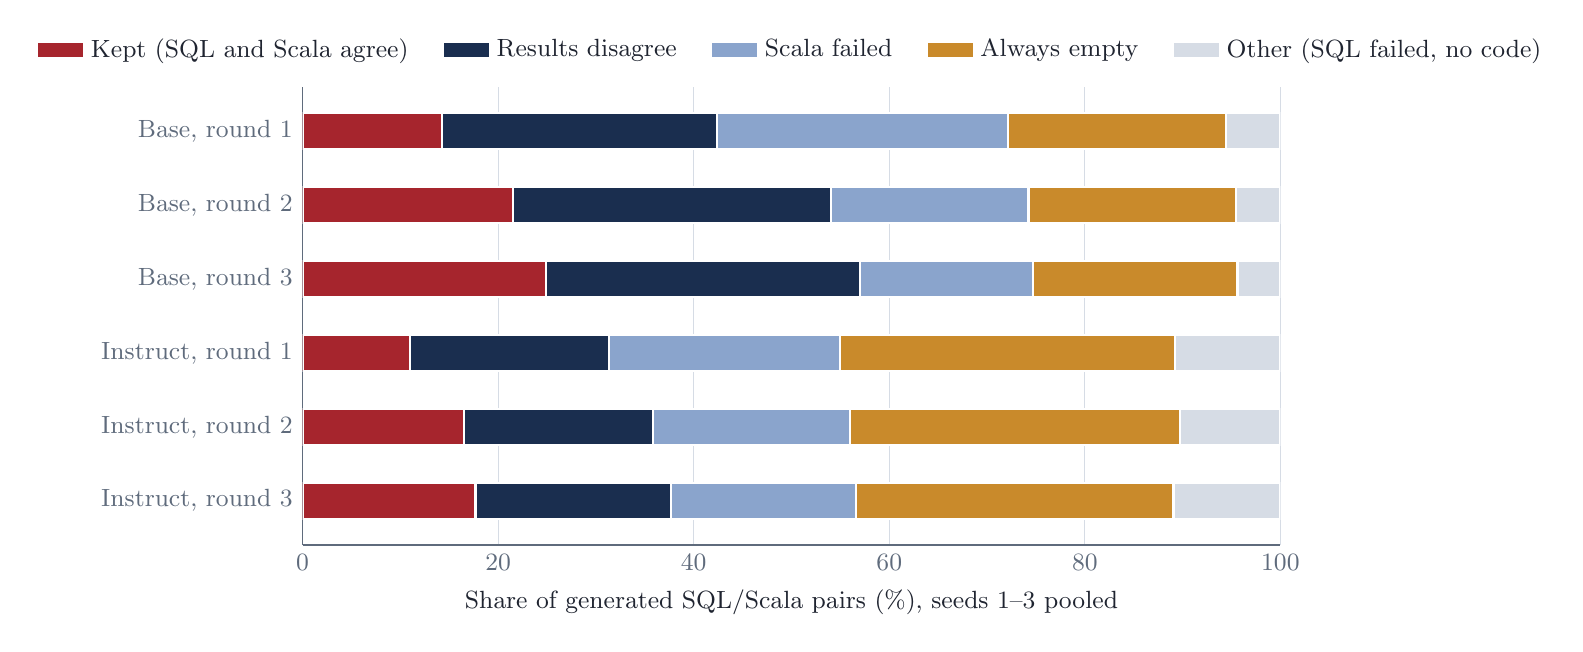
\begin{tikzpicture}
\begin{axis}[rd, xbar stacked, bar width=13pt, width=14cm, height=7.4cm, ymajorgrids=false, xmajorgrids,
  xmin=0, xmax=100, ytick={0,...,5}, yticklabels={{Instruct, round 3},{Instruct, round 2},{Instruct, round 1},{Base, round 3},{Base, round 2},{Base, round 1}}, ymin=-0.6, ymax=5.6,
  xlabel={Share of generated SQL/Scala pairs (\%), seeds 1--3 pooled}, xtick={0,20,...,100},
  legend style={at={(0.5,1.03)},anchor=south,legend columns=5}, every axis plot/.append style={draw=white,line width=0.8pt}]
\addplot[area legend,fill=tsred] coordinates {(17.69,0) (16.49,1) (10.99,2) (24.93,3) (21.56,4) (14.24,5)};
\addplot[area legend,fill=tsnavy] coordinates {(19.98,0) (19.38,1) (20.33,2) (32.10,3) (32.50,4) (28.11,5)};
\addplot[area legend,fill=cVanPaper] coordinates {(18.89,0) (20.10,1) (23.62,2) (17.69,3) (20.19,4) (29.80,5)};
\addplot[area legend,fill=cControl] coordinates {(32.51,0) (33.79,1) (34.32,2) (20.89,3) (21.19,4) (22.30,5)};
\addplot[area legend,fill=tsline] coordinates {(10.93,0) (10.24,1) (10.75,2) (4.38,3) (4.56,4) (5.55,5)};
\node[font=\scriptsize\bfseries,text=white,anchor=west] at (axis cs:0.6,0) {18\%};
\node[font=\scriptsize\bfseries,text=white,anchor=west] at (axis cs:0.6,1) {16\%};
\node[font=\scriptsize\bfseries,text=white,anchor=west] at (axis cs:0.6,2) {11\%};
\node[font=\scriptsize\bfseries,text=white,anchor=west] at (axis cs:0.6,3) {25\%};
\node[font=\scriptsize\bfseries,text=white,anchor=west] at (axis cs:0.6,4) {22\%};
\node[font=\scriptsize\bfseries,text=white,anchor=west] at (axis cs:0.6,5) {14\%};
\legend{Kept (SQL and Scala agree),Results disagree,Scala failed,Always empty,{Other (SQL failed, no code)}}
\end{axis}
\end{tikzpicture}
\end{document}
